\chapter{\ChapterTwo{}} \label{amigo}
%\lhead{\emph{\ChapterTwo{}}}

En este capítulo procederemos a explicar el caso de estudio escogido para el desarrollo del trabajo, así como la problemática asociada y las soluciones implementadas para el desarrollo de la misma.

\section{Descripción del caso de estudio}

El caso de estudio escogido consiste en la clasificación de los Trabajos de Fin de Grado (TFGs) que se encuentran en el Repositorio Institucional de la ULL, partiendo de la información que se puede recabar sobre los mismos.
%
El objetivo de este caso de estudio es el de obtener un sistema de clasificación de TFGs que pueda servir como suplemento a la hora de asignar un área temática a un TFG cuando éste es inscrito a la plataforma.

\section{Opciones de clasificación}

La clasificación de textos es un subproblema del campo del Procesamiento del Lenguaje Natural, entre muchos otros como aquéllos discutidos en el capítulo anterior (\ref{amigo}).
%
Fue escogido debido a la facilidad y rapidez de su implementación con las herramientas disponibles a día de hoy, entre ellas el NLTK.
%
Existen varias formas de realizar la clasificación de un texto, todas claramente atendiendo a las características del mismo, pero utilizando diferentes enfoques.
%
En las siguientes secciones pasamos a describir los enfoques más utilizados para ello.

\subsection{Enfoques estadísticos}

Esta clase de enfoques hacen uso de las técnicas de Aprendizaje Automático, que hoy en día son las que gozan de mayor aceptación y crecimiento.
%
Utilizan técnicas estadísticas para realizar estimaciones sobre un conjunto de datos del que se desconoce una o varias características, y se procede a asignar
%
El éxito de este tipo de técnicas se basa en las características que sean detectadas y seleccionadas como relevantes para el problema de clasificación que se tenga.

\begin{minipage}{\linewidth}
\textit{Tomemos como ejemplo un hipotético estudio sobre los hábitos alimenticios de un grupo de animales.
El color del pelaje de un animal no es relevante a la hora de inferir su dieta, pero en cambio la clase de dentadura que posea sí lo es. Por tanto, en este caso se deberá ignorar el color del pelaje pero tomar en cuenta el tipo de dentadura de los animales.}
\end{minipage}

%Por tanto, es 

Para los casos de aprendizaje supervisado, existen elementos ya clasificados de manera correcta, ya sea por parte de otro programa o de manera manual. Estos elementos son utilizados para conformar un subconjunto de entrenamiento.

En estos casos de aprendizaje supervisado, es importante cuidarse de no sobreajustar el clasificador a la clasificación de los problemas de entrada. 
%
El problema del sobreajuste es un problema difícil de resolver objetivamente, y suele manejarse mejor cuando se tiene un cierto nivel de experiencia en tratar con él.

En el caso del aprendizaje no supervisado, no se poseen de datos de entrenamiento, por lo que normalmente recae sobre el algoritmo la diferenciación de los elementos en diferentes clases \say{a posteriori}, es decir, clases que no habían sido definidas antes de la tarea de clasificación.

%Este método puede brindar nuevas maneras de...

%Uno de los problemas que tiene esta clase de enfoque es que muchas veces no proporciona un modelo claro, con algunas excepciones, de la lógica utilizada para clasificar los textos.

%Las excepciones a la regla son los árboles de clasificación, que pueden ser utilizados una vez se conoce la estructura del problema.
%Si se desconoce la estructura del problema pero en cambio se tienen datos etiquetados, pueden ser generados mediante técnicas de Aprendizaje Automático.

\subsection{Naive Bayes}

Los clasificadores de Bayes ingenuos (\textit{Naive Bayes classifiers}) son clasificadores utilizados ampliamente en la actualidad para problemas de clasificación de textos, tanto en ámbitos académicos como industriales.

Los caracteriza una gran simplicidad, que conlleva la ventaja de que son de fácil comprensión y por tanto de fácil uso.

A pesar de esta simplicidad, los clasificadores de Bayes ingenuos son bastante eficaces y tienen una gran cantidad de aplicaciones prácticas.

Los clasificadores de Bayes ingenuos se basan en un modelo probabilístico, el Teorema de Bayes.

\begin{equation}\label{eq:bayes}
    p(C_k|x) = \frac{p(C_k)p(x|C_k)}{p(x)}
\end{equation}

Según este teorema, la probabilidad de un suceso $C_k$, dada una situación $x$ viene determinada por el número de veces que se ha producido el suceso $C_k$ en esa situación $x$, dividido por el número de veces total que se ha encontrado esta situación $x$
(Eq. \ref{eq:bayes}).

Aplicados al problema de la clasificación, nos permite inferir la posibilidad que tiene un elemento de pertenecer a cada una de las clases consideradas, teniendo en cuenta cada una de las características de este elemento como un suceso a priori.

Los clasificadores de Bayes ingenuos reciben su nombre debido a que toman en cuenta la contribución de cada característica hacia la posibilidad de una clasificación de manera independiente, en contraposición a correlacionar varias características para realizar una estimación más precisa a la hora de clasificar un elemento.

\subsection{Enfoques analíticos}

\lhead{\emph{\ChapterTwo{}}}
Los enfoques analíticos son aquéllos que intentan realizar un análisis morfosintáctico sobre el texto de entrada, obteniendo información relativa a las construcciones sintácticas de las oraciones y la morfología de las palabras utilizadas.
%
Esta clase de enfoques se basa en el análisis morfosintáctico clásico, que lleva realizándose durante siglos de forma manual, como herramienta docente para dar a conocer las bases de un lenguaje natural.

Sin embargo, se trata de enfoques de mayor complejidad en comparación con los enfoques estadísticos, debido a que requieren la implementación de conocimientos sobre la gramática, sintaxis y semántica del lenguaje objetivo.
%
Por ejemplo se deben de conocer todas las conjugaciones posibles de todos los verbos del lenguaje objetivo, y atender al contexto de las oraciones para utilizar la acepción correcta de palabras ambigüas.

Por otra parte, las herramientas de PLN deben contener corpus morfosintácticos y semánticos para cada uno de los idiomas, además de requerir para cada uno de ellos diferente para paliar las idiosincracias de cada uno de los lenguajes.

Debido a estas razones, y con motivo de atenerse al tiempo disponible, se ha decidido no adentrarnos en esta clase de análisis, que sin embargo resulta bastante prometedor.

\section{Trabajos de Fin de Grado en la ULL: ¿Qué revela el análisis automático de texto sobre los mismos?}
En nuestro caso de estudio, se utilizó como fuente el Repositorio Institucional de la Universidad de La Laguna (RIULL), conteniendo ésta los documentos que se deseaban explotar.
%
Se ha realizado un desarrollo en base a aproximaciones, cada una de ellas con resultados que han sido comparados entre sí para constatar su eficacia.

\subsection{Obtención de datos}
\lhead{\emph{\ChapterTwo{}}}
%\section{Obtención de datos}

El primer paso para realizar el Procesamiento del Lenguaje Natural consiste en obtenerlo. Normalmente se busca extraer información de una fuente para poder explotarla y obtener el texto a procesar.
%
En nuestro caso de estudio, la obtención de información se centró en los Trabajos de Fin de Grado (TFG), usando como fuente de información el Repositorio Institucional de la Universidad de La Laguna (RIULL).
%
El procedimiento utilizado para la obtención de información referente a estos documentos fue el uso de una herramienta de \textit{web scraping} sobre la página web de la RIULL, cuyo uso se explica a continuación.
%Se consideró descargar los Trabajos de Fin de Grado (TFG) en formato PostScript (extensión ".pdf"), lo que luego fue descartado debido a ...

\subsection{Obtención de datos con CasperJS}

% Como se explicó en el anterior capítulo, se consideró descargar los Trabajos de Fin de Grado en formato PDF, lo que luego fue descartado debido al alto coste de procesar una gran cantidad de PDFs y el hecho de tener que implementar una herramienta de transformación a texto plano en la cadena de automatización de procesamiento de texto.

% Otra razón por la cual fue descartada la extracción de texto a partir de PDF es la imperfección de las herramientas actuales de transcripción de PDF generales, por lo que habría hecho falta la adaptación de un programa similar que considerase las características particulares de los trabajos de fin de grado del caso de estudio, lo que no se mostró como una opción práctica a la hora de realizar el estudio.

El proceso de obtención de datos se basó en el uso de la herramienta software CasperJS \cite{casperjs} para simular una navegación y recabar datos de las páginas web del RIULL de manera automatizada.
%
La herramienta actúa de la misma manera que un navegador de uso personal, enviando peticiones HTTP, recibiendo información y prosiguiendo de la manera que se le haya indicado.
En este caso se implementó la recogida de datos partiendo de la página en la que se muestran los TFG por orden de publicación, y se realiza la paginación hasta haber recuperado los enlaces individuales para cada uno de los TFG.

Es entonces cuando se procede a la extracción de los metadatos de cada página individual de TFG, obteniendo los datos relevantes de cada TFG como su título, descripción y clasificación.

\subsection{Extracción de la información}

CasperJS trabaja mediante la ejecución de un \textit{script}(guión) en lenguaje JavaScript, que le es proporcionado como entrada.


\lhead{\emph{\ChapterFour{}}}
\lstset{
   language=Javascript
}

Antes que nada, se debe crear una instancia del navegador CasperJS, incorporando la librería \textit{casper} y pasando las opciones de creación como argumento.

\begin{center}
\begin{minipage}{\linewidth}
% \label{fig:code01}
\begin{lstlisting}[caption=Creación del navegador CasperJS.]
var casper = require('casper').create({
//  verbose: true,
  logLevel: "debug"
});
\end{lstlisting}
\end{minipage}
\end{center}



\todo{
\begin{codigo}
definir entorno de codigo
\end{codigo}
}

En este caso se le pasa el argumento \textit{verbose} para indicar que se desea que muestre mensajes informativos al realizar las acciones que se le pasen, mientras que el argumento \textit{logLevel} sirve para especificar el detalle que precisamos de esos mensajes. %(Fig. \ref{fig:code01}).

\begin{center}
\begin{minipage}{\linewidth}
\begin{lstlisting}[caption=Estructuras de datos para la navegación por la página.]
// Enlaces hacia las paginas de los TFGs.
var links = [];
// Offset navegado hasta el momento en el catalogo de TFGs.
var offset = 0;
\end{lstlisting}
\end{minipage}
\end{center}

El navegador obtendrá los enlaces a cada página individual de TFG, los cuales deberá mantener en memoria hasta la finalización de la ejecución del programa de extracción de datos.
Es por ello que se define la variable \textit{enlaces} que los contendrá. Por otra parte, al realizar el paginado se debe conocer la posición del navegador de manera inmediata, por lo que se mantiene y actualiza en la variable \textit{offset}. %(Fig. \ref{fig:code02}).

\begin{center}
\begin{minipage}{\linewidth}
\begin{lstlisting}[caption=Estructuras de datos para las características de cada TFG.]
var titles = [];
var descriptions = [];
var tags = [];
\end{lstlisting}
\end{minipage}
\end{center}

Las características que se han tomado como relevantes en la primera aproximación han sido el título, la descripción y las etiquetas que se han dado a cada TFG en el repositorio. Estas se mantendrán en variables separadas. %(Fig. \ref{fig:code03}).

\begin{center}
\begin{minipage}{\linewidth}
\begin{lstlisting}[caption=Función de obtención de enlaces individuales.]
// En cualquier pagina de TFGs recientes de un grado,
// obtener los enlaces a las paginas de los TFGs.
function scrapeLinks() {
    var links = $('li.ds-artifact-item a');
    return Array.prototype.map.call(links, function(e) {
        return e.getAttribute('href');
    });
}
\end{lstlisting}
\end{minipage}
\end{center}

Durante la paginación, cada una de las páginas muestra enlaces individuales hacia cada uno de los Trabajos de Fin de Grado. Para ello, estando el navegador en cualquier página del catálogo, obtenemos los elementos \textit{href} y con ellos todos los enlaces de la vista actual. %(Fig. \ref{fig:code04}).

\begin{center}
\begin{minipage}{\linewidth}
\begin{lstlisting}[caption=Función de paginado.]
// Estando en el catalogo, obtiene el enlace a
// la siguiente pagina del catalogo si la hay.
function scrapeNextPageLink(){
  if ($('.next.pull-right.disabled').length > 0) return null;
  return $('a.next-page-link')[0].href;
}
\end{lstlisting}
\end{minipage}
\end{center}

Durante la paginación, se debe conocer si existe una página subsecuente a aquélla en la que se encuentra el navegador actualmente. Para ello inspeccionamos si el botón que permite paginar a la siguiente página está bloqueado en la vista. De ser este el caso, nos encontramos en la última página. De otro modo, conseguimos el nuevo enlace del elemento de paginación. %(Fig. \ref{fig:code05}).

\begin{center}
\begin{minipage}{\linewidth}
\begin{lstlisting}[caption=Función de obtención de todos los enlaces de TFG.]
/**
* Obtiene todos los enlaces de los TFGs de un Grado.
* Se presupone que Casper se encuentra en
* la primera pagina de TFGs recientes del Grado.
*/
function casperLinksOnThisBachelor(){
    var newLinks = casper.evaluate(scrapeLinks);
    links = links.concat(newLinks);
    var nextLink = casper.evaluate(scrapeNextPageLink);

    casper.echo('nextLink: ' + nextLink);
    if (nextLink) {
        // casper.thenClick(nextLink);
        casper.thenOpen(nextLink);
        casper.then(casperLinksOnThisBachelor);
    } else {
        casper.echo("END");
    }
}
\end{lstlisting}
\end{minipage}
\end{center}

Aplicamos las anteriores funciones en lo que viene a ser el bucle principal del programa, una función recursiva que se detiene cuando el navegador ha llegado a la última página.

\begin{center}
\begin{figure}[!ht]
  \caption{Vista en la que se muestran los metadatos de un TFG.}
  \label{fig:metadata_view}
  \centering
    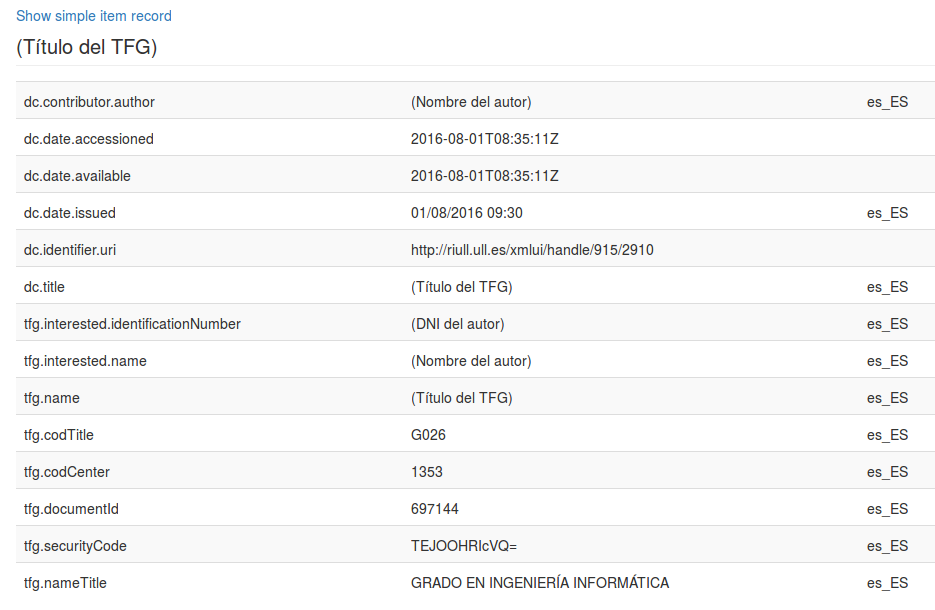
\includegraphics[width=0.8\textwidth]{Images/metadata_view}
\end{figure}
\end{center}

\begin{center}
\begin{minipage}{\linewidth}
\begin{lstlisting}[caption=Función de obtención de metadato por nombre de etiqueta.]
// En una pagina del TFG, obtener el valor del campo 'str' (si lo hay).
function scrapePageValue(str){
    var datum = $('td.label-cell:contains(' + str + ') + td')[0].innerHTML;
    if (datum === null || datum === undefined || datum === "")
        datum = "---";
    return datum;
}
\end{lstlisting}
\end{minipage}
\end{center}

Esta función se basa en la vista de la página para obtener el texto perteneciente a una etiqueta. Por ejemplo, para el caso de la Fig.\ref{fig:metadata_view}, si se le pasa \texttt{author} obtendrá \texttt{(Nombre del autor)}.

% En caso de que no exista, la función devolverá una cadena estándar (en este caso "\texttt{---}") para evitar romper el flujo del programa.

\begin{center}
\begin{minipage}{\linewidth}
\begin{lstlisting}[caption=Función de obtención de metadatos por nombre de etiqueta similar.]
// En una pagina del TFG, obtener el valor de varios campos 'str' (si los hay).
function scrapePageValues(str){
    var data = $('td.label-cell:contains(' + str + ') + td');
    var data2 = [];
    for (var i = 0; i < data.length; i++){
      data2.push(data[i].innerHTML);
    }
    if (data2.length < 1) data2.push("---");
    return data2;
}
\end{lstlisting}
\end{minipage}
\end{center}

Definimos además una función similar a la anterior, con la diferencia de que inspecciona la página para encontrar múltiples datos definidos bajo el mismo nombre. Esto es importante dado que existen metadatos que están definidos bajo campos de mismo nombre, por ejemplo: dos campos de "tema" con distintos valores para expresar que un TFG forma parte de múltiples temas.

\begin{center}
\begin{minipage}{\linewidth}
\begin{lstlisting}[caption=Función de concatenación de enlace.]
function completeLink(currentValue, index, array){
  return 'http://riull.ull.es'.concat(currentValue).concat('?show=full');
}
\end{lstlisting}
\end{minipage}
\end{center}

% Uno de los problemas fue la imposibilidad de realizar una recurrencia sin blabla, por eso se recurrió a crear una función externa

\begin{center}
\begin{minipage}{\linewidth}
\begin{lstlisting}[caption=Función tipo que permite la recurrencia con CasperJS.]
function functionOutsideLoop(){
  links.concat(casper.evaluate(scrapeLinks));
}
\end{lstlisting}
\end{minipage}
\end{center}


%Como primer paso, se le proporciona al navegador CasperJS la página inicial, hacia la cual deberá navegar para iniciar el proceso de extracción. En este caso, es la página que muestra los Trabajos de Fin de Grado para los alumnos del Grado de Informática.

%Una vez en la página de los trabajos de fin de grado, el navegador CasperJS fue programado para obtener los enlaces que le llevarían a las páginas individuales de cada uno de los TFG.

\subsection{Almacenamiento de la información}
\lhead{\emph{\ChapterTwo{}}}
%\subsection{Almacenamiento de la información}
Se decidió guardar la información obtenida del proceso de extracción de texto en archivos locales en el disco duro del ordenador utilizado para la realización del trabajo.

El formato utilizado para los archivos de texto es CSV (\textit{Comma Separated Values}), es decir, archivos de texto planos-
%
Se trata de un formato sencillo en el cual cada elemento se encuentra en una línea diferente, y las características de dichos elementos separados por comas.

La razón por la que se utilizó éste formato se debe a la mayor comodidad que aporta en un caso de estudio restringido, con una cantidad de datos relativamente pequeña.
%
Otra razón por la que se eligió el formato CSV es la disponibilidad de librerías Python que trabajan en este formato, incrementando la facilidad y rapidez de desarrollo del sistema de almacenamiento.

\subsection{Clasificación del texto}
\lhead{\emph{\ChapterFour{}}}

\lstset{
   language=Python
}

\begin{minipage}{\linewidth}
\begin{lstlisting}[caption=Función para cargar instancias de un archivo CSV.]
def cargar_instancias_de_csv(ruta, formato=None):
    """
    Cargamos las instancias de un archivo CSV.

    :param ruta: Ruta del archivo csv que se leerá.
    :param formato: Formato 
    :return: Una lista con cada una de las filas del csv.
    """
    instancias = []
    with open('tfg.csv') as csvfile:
        reader = csv.DictReader(csvfile)
        for row in reader:
            instancias.append((row['Clasificación'], row['Título'], row['Descripción']))
    return instancias
}
\end{lstlisting}
\end{minipage}